\section{Head-to-head comparison under the shared protocol}
\label{sec:comparison}

This section contains the central results of the paper: all four methods, reduced to per-class binary masks, scored with identical metrics on the identical spatially disjoint validation tiles (Sect.~\ref{sec:metrics_protocol}). The comparison is organised per class, because the two classes with usable supervision pose opposite problems: \texttt{impact\_crater} is nearly saturated (prevalence 0.82) while \texttt{wrinkle\_ridge} is sparse (prevalence 0.0064) but genuinely learnable.

\subsection{Impact crater: the base-rate regime}
\label{sec:comp_crater}

On the full spatial validation set the crater channel covers 82\% of pixels, and a \emph{predict-everything} baseline attains F1 $=0.90$ and IoU $=0.82$ with MCC $=0$. Table~\ref{tab:crater_allval} shows that the SmallUNet essentially reproduces this baseline (F1 $=0.90$, MCC $=0.01$): its high F1 is not evidence of skill --- the network has learned to output the base rate, which on a channel where 50.7\% of tiles contain no negative pixels at all (Table~\ref{tab:prevalence}) is very hard to beat. Any comparison ranking methods by F1 or IoU here would be ranking base-rate reproduction; this is why MCC is the protocol's primary metric.

\begin{table}[htbp]
\centering
\caption{Impact crater, full spatial validation set (per-method calibrated threshold $\tau$). The predict-all row labels every pixel crater. MCC is the primary ranking metric; F1/IoU are dominated by the 0.82 base rate.}
\label{tab:crater_allval}
\resizebox{\columnwidth}{!}{%
\begin{tabular}{lrrrrrr}
\toprule
Method & $\tau$ & Precision & Recall & F1 & IoU & MCC \\
\midrule
YOLOv8 (detection)     & 0.2  & 0.893 & 0.940 & 0.916 & 0.846 & \textbf{0.470} \\
Classical (thr+morph)  & 0.5  & 0.878 & 0.238 & 0.374 & 0.230 & 0.078 \\
SmallUNet (semantic)   & 0.3  & 0.823 & 1.000 & 0.903 & 0.823 & 0.013 \\
Mask R-CNN (instance)  & 0.05 & 0.616 & 0.064 & 0.116 & 0.061 & $-0.166$ \\
\midrule
Predict-all (baseline) & ---  & 0.823 & 1.000 & 0.903 & 0.823 & 0.000 \\
\bottomrule
\end{tabular}
}
\end{table}

Partitioning the validation tiles by crater coverage (Table~\ref{tab:crater_regime}, Fig.~\ref{fig:regime}) shows that the best method \emph{flips} with the regime. On crater-sparse tiles (1--20\% coverage), where craters are countable objects, the instance and detection formulations lead: Mask R-CNN (MCC 0.19) ahead of YOLOv8 (0.16), with the classical baseline modest (0.07) and the SmallUNet at chance. On crater-dense tiles ($\geq$20\%), where the channel is a coverage layer, YOLOv8 keeps a positive signal (0.24) while Mask R-CNN collapses ($-0.11$; such tiles are out of distribution for its instance-target preparation, which skips channels above 20\% coverage, Sect.~\ref{sec:maskrcnn}), and the SmallUNet remains at chance in \emph{both} regimes. One caveat: MCC and F1 at a fixed operating point are sensitive to the calibrated threshold, so absolute values shift with $\tau$; the rankings and the regime flip are stable across the calibration range we scanned.

\begin{table}[htbp]
\centering
\caption{Impact crater by coverage regime (spatial validation split; per-method, per-regime calibrated $\tau$). The preferable formulation flips between regimes.}
\label{tab:crater_regime}
\resizebox{\columnwidth}{!}{%
\begin{tabular}{llrrrr}
\toprule
Regime & Method & $\tau$ & F1 & MCC & Count MAE \\
\midrule
sparse (1--20\%, $n=94$)  & Mask R-CNN & 0.2  & 0.279 & \textbf{0.187} & 82.8 \\
                          & YOLOv8     & 0.05 & 0.253 & 0.159 & 105.5 \\
                          & Classical  & 0.5  & 0.142 & 0.069 & 15.6 \\
                          & SmallUNet  & 0.3  & 0.176 & $-0.000$ & 24.0 \\
\midrule
dense ($\geq$20\%, $n=192$) & YOLOv8     & 0.1  & 0.947 & \textbf{0.240} & 12.6 \\
                          & Classical  & 0.5  & 0.387 & 0.031 & 49.3 \\
                          & SmallUNet  & 0.3  & 0.945 & $-0.001$ & 4.9 \\
                          & Mask R-CNN & 0.05 & 0.132 & $-0.111$ & 41.3 \\
\bottomrule
\end{tabular}
}
\end{table}

\begin{figure}[htbp!]
\centering
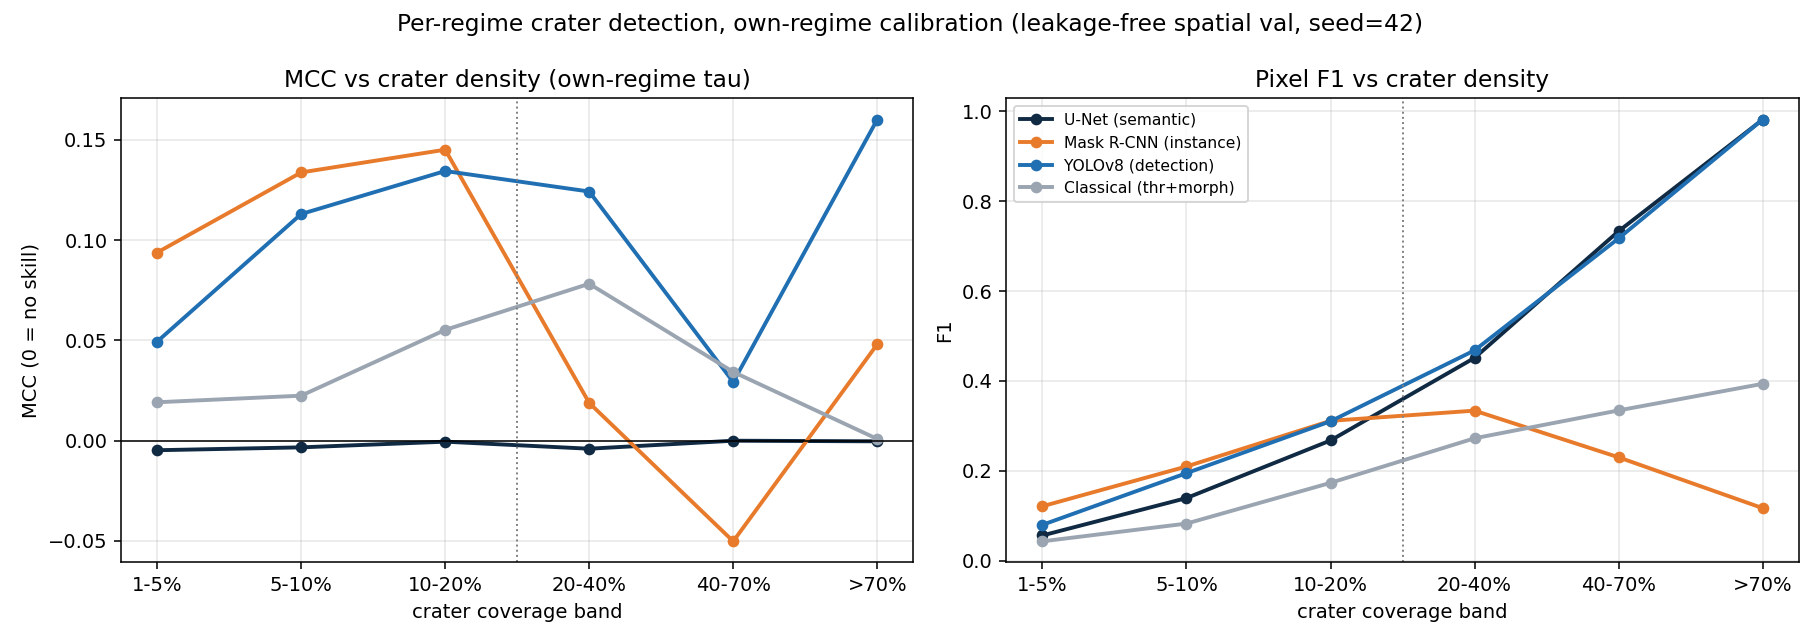
\includegraphics[width=\columnwidth,keepaspectratio]{figures/comparison/fig_regime.png}
\caption{Impact-crater comparison by coverage regime on the spatial validation split. Left: MCC (skill over base rate); right: F1 for reference. The ranking flips between regimes, and the SmallUNet sits at MCC $\approx0$ in both --- its high F1 on dense tiles is base-rate reproduction, not detection skill.}
\label{fig:regime}
\end{figure}

\subsection{Wrinkle ridge: the class with genuine signal}
\label{sec:comp_ridge}

Wrinkle ridges are the mirror image of craters: prevalence 0.0064, so chance-level performance is near zero and any positive score reflects learned structure. The comparison runs on the 524 ridge-bearing tiles of the spatial validation split (210 calibration / 314 test); the SmallUNet entry is the definitive no-augmentation spatial checkpoint of Sect.~\ref{sec:mr_augmentation}, the YOLOv8 entry the committed ridge-focused six-class model, and the classical entry the Sato filter of Sect.~\ref{sec:classical}.

\begin{table}[htbp]
\centering
\caption{Wrinkle ridge, spatial validation split (314 test tiles, per-method calibrated $\tau$). Prevalence 0.0064: chance-level MCC is 0, and the predict-all baseline collapses.}
\label{tab:ridge}
\resizebox{\columnwidth}{!}{%
\begin{tabular}{lrrrrrr}
\toprule
Method & $\tau$ & Precision & Recall & F1 & MCC & ms/tile \\
\midrule
SmallUNet (semantic)   & 0.25 & 0.527 & 0.409 & \textbf{0.460} & \textbf{0.452} & 20 \\
Mask R-CNN (instance)  & 0.5  & 0.414 & 0.352 & 0.380 & 0.366 & 1130 \\
YOLOv8 (detection)     & 0.01 & 0.063 & 0.228 & 0.099 & 0.076 & 10 \\
Classical (Sato)       & 0.05 & 0.021 & 0.392 & 0.040 & $-0.028$ & 29 \\
\midrule
Predict-all (baseline) & ---  & 0.026 & 1.000 & 0.050 & 0.000 & --- \\
\bottomrule
\end{tabular}
}
\end{table}

\begin{figure}[htbp!]
\centering
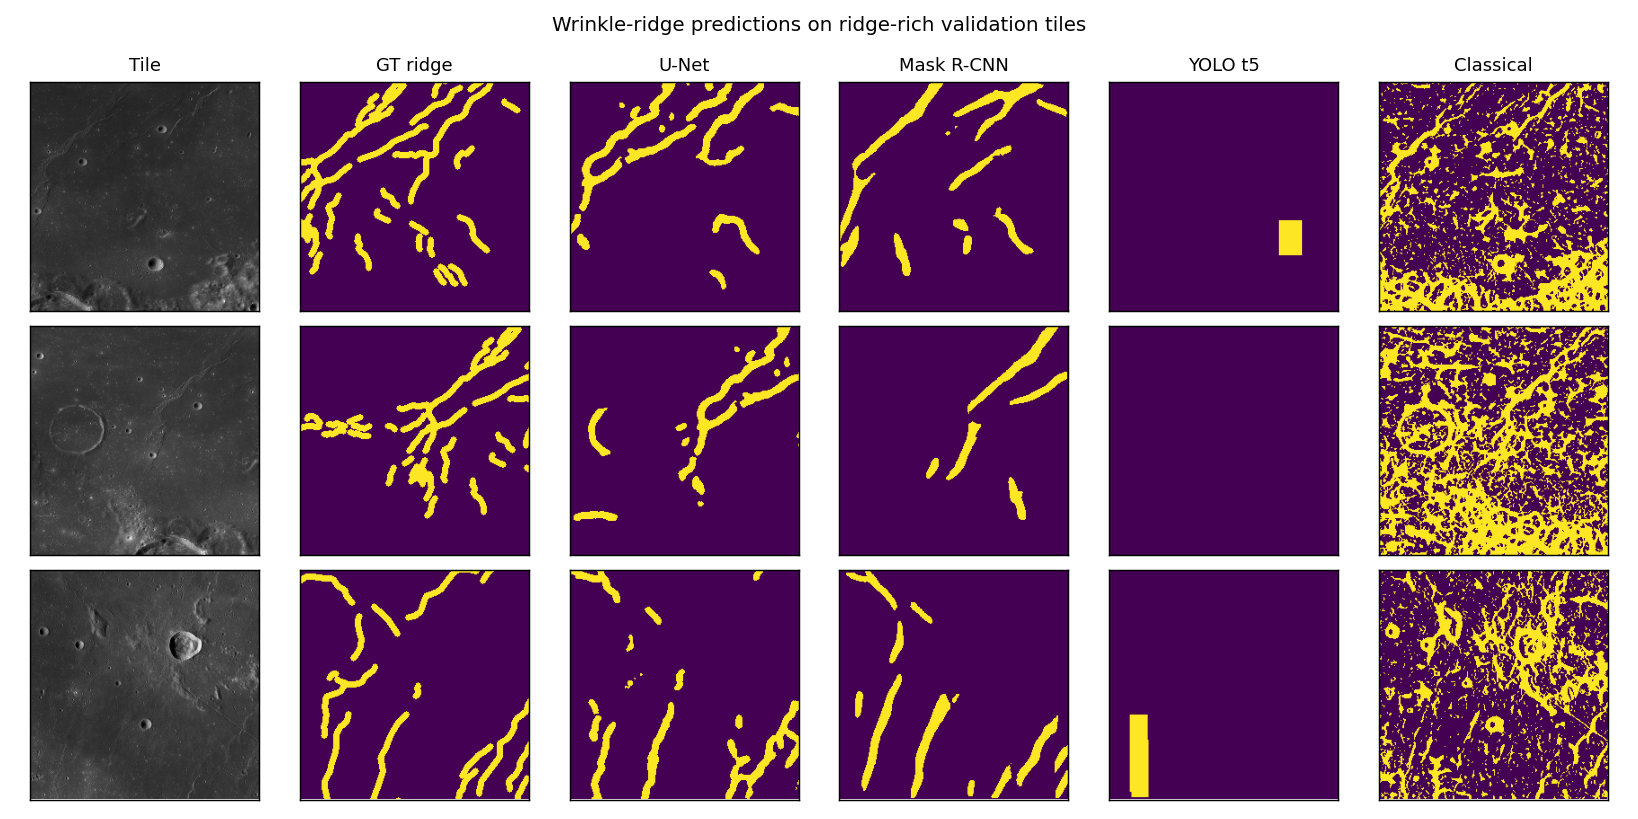
\includegraphics[width=\columnwidth,keepaspectratio]{figures/comparison/fig_ridge_qualitative.png}
\caption{Qualitative ridge predictions on common validation tiles (columns: image, ground truth, then one column per method). The SmallUNet recovers the connected ridge network; Mask R-CNN recovers the strongest segments; YOLOv8 boxes are coarse; the Sato filter responds to every elongated bright structure, ridge or not.}
\label{fig:ridge_qual}
\end{figure}

The ranking reverses relative to the sparse-crater regime: \textbf{SmallUNet (MCC 0.452) $>$ Mask R-CNN (0.366) $\gg$ YOLOv8 (0.076) $>$ Sato ($\approx$ chance)} (Table~\ref{tab:ridge}, Fig.~\ref{fig:ridge_qual}). The two pixel-supervised models are far ahead, consistent with the nature of the class: ridges are thin, extended, and connected --- pixel supervision describes them well, whereas a diagonal ridge fills a small fraction of its own bounding box. The SmallUNet additionally beats Mask R-CNN at ${\sim}1/60$th of the inference cost, and the context-free classical filter stays at chance. Together with Sect.~\ref{sec:comp_crater} this yields the central per-class conclusion: \emph{semantic segmentation wins where dense pixel supervision exists; instance detection wins for sparse countable objects; nothing wins on a saturated channel.}

\subsection{Effect of the split protocol: a controlled study}
\label{sec:split_study}

To quantify what the split choice does to a reported number, we retrained \emph{identical} single-class YOLOv8n detectors (image size 256, batch 16, 40 epochs, identical seeds and hyperparameters) on datasets built by the same box-extraction code, changing \emph{only} the split: random 80/20 tile split versus spatial block split, with comparable training volumes in both arms (crater: 5\,659 vs.\ 5\,077 tiles; ridge: 2\,339 vs.\ 2\,202). We report each model on its own validation set, plus a decomposition row --- the random-split model evaluated on the \emph{spatial} validation tiles --- which separates the training-side from the evaluation-side component of the leakage.

\begin{table}[htbp]
\centering
\caption{Split-protocol study: identical YOLOv8n detectors, identical budget (40 epochs), different train/validation split. ``Random $\to$ spatial'' evaluates the random-split model on the spatial validation tiles.}
\label{tab:split_study}
\resizebox{\columnwidth}{!}{%
\begin{tabular}{llrrr}
\toprule
Class & Protocol & mAP50 & Precision & Recall \\
\midrule
impact crater & random tile split (own val) & 0.122 & 0.217 & 0.222 \\
              & spatial split (own val)     & 0.106 & 0.206 & 0.201 \\
              & random $\to$ spatial val    & 0.129 & 0.228 & 0.219 \\
\midrule
wrinkle ridge & random tile split (own val) & 0.146 & 0.297 & 0.191 \\
              & spatial split (own val)     & 0.077 & 0.203 & 0.130 \\
              & random $\to$ spatial val    & 0.117 & 0.278 & 0.162 \\
\bottomrule
\end{tabular}
}
\end{table}

Both classes replicate the effect, with strongly class-dependent size (Table~\ref{tab:split_study}). For wrinkle ridges the protocol choice alone nearly doubles the reported score: mAP50 0.146 (random) against 0.077 (spatial) for an identical model, budget, and pipeline. The decomposition row separates the contributions: on \emph{identical} validation tiles the random-trained model outscores the spatial-trained one (0.117 vs.\ 0.077) --- a training-side contamination benefit of $+0.040$, since its training set contains tiles overlapping the validation blocks --- while the remaining $+0.029$ (0.146 vs.\ 0.117) is the evaluation-side component, the random protocol's own validation tiles sharing half their pixels with training tiles. For craters the total effect is much smaller (0.122 vs.\ 0.106): the near-saturated channel offers little memorisable detail that is not already ubiquitous.

Extending the ridge pair to 150 epochs (Fig.~\ref{fig:split_divergence}) confirms the budget dependence: the random-split curve climbs monotonically (0.146 at epoch 40, 0.217 at 150, still rising) while the spatial-split curve saturates before epoch 40 in the 0.06--0.08 band, so the gap \emph{grows} with training --- from $\times1.9$ to $\times2.6$ --- as additional epochs memorise near-duplicate content while genuine generalisation stopped improving long before. Two consequences follow. First, random-split scores on this dataset are not comparable to spatial ones, and the discrepancy is largest exactly where detection genuinely works; development-time scores quoted at large budgets under random splits (Sect.~\ref{sec:yolo_ensemble}) therefore overstate generalisation increasingly with budget. Second, the honest absolute level matters for Sect.~\ref{sec:comp_ridge}: the dedicated single-class ridge detector under the spatial protocol (mAP50 0.077) is fully consistent with the six-class model's shared-protocol showing (MCC 0.076) --- YOLO's weakness on ridges is a property of the box representation on curvilinear features, not an artefact of one training run.

\begin{figure}[htbp!]
\centering
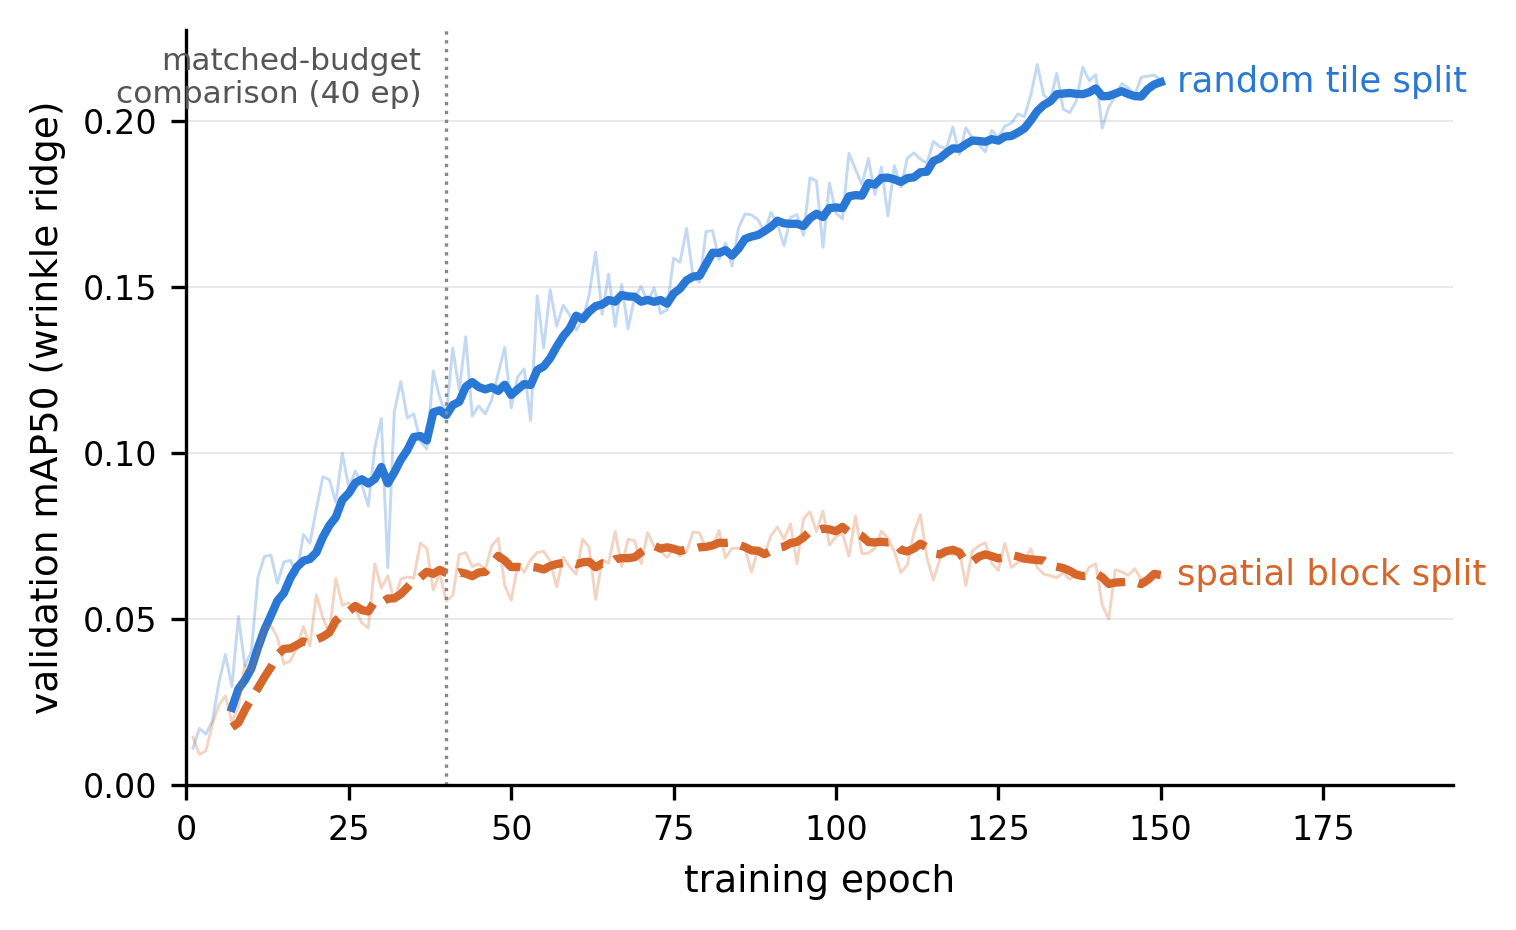
\includegraphics[width=\columnwidth,keepaspectratio]{figures/comparison/fig_split_divergence.png}
\caption{Validation mAP50 of the single-class wrinkle-ridge detector over 150 epochs under the two split protocols (thin: per-epoch; thick: 7-epoch rolling mean; dotted: the matched-budget comparison of Table~\ref{tab:split_study}). The random-split curve keeps climbing as training memorises near-duplicate tiles; the spatial-split curve --- true generalisation --- plateaus before epoch 40. A leaky protocol plus a long training run can report an arbitrarily inflated score.}
\label{fig:split_divergence}
\end{figure}

\subsection{Trade-offs beyond accuracy}
\label{sec:tradeoffs}

Accuracy is one axis; Table~\ref{tab:ridge} also reports cost. Mask R-CNN pays ${\sim}1.1$\,s per tile on CPU --- a full south-pole pass takes over an hour, versus about a minute for the SmallUNet and YOLOv8 and seconds for the classical baseline. Data-preparation effort differs as sharply: the segmentation networks consume the semantic masks directly, while both detection methods depend on a semantic-to-instance conversion whose noise propagates into training targets (Sect.~\ref{sec:maskrcnn}). Interpretability runs in the opposite direction: every classical parameter has physical meaning, detector boxes are auditable object by object, and dense probability maps require post-hoc threshold calibration. None of these axes changes the per-class accuracy ranking, but they decide deployability: for survey-scale mapping of ridge-like features the SmallUNet offers the best accuracy-per-cost, while for counting sparse objects Mask R-CNN's lead costs two orders of magnitude more compute.
